\documentclass[a4paper]{article}
\usepackage[T1]{fontenc}
\usepackage[utf8]{inputenc}
\usepackage[english]{babel}
\usepackage{graphicx}
\usepackage{float}
\usepackage{graphicx}
\usepackage{hyperref}
\usepackage{makeidx}
\usepackage{caption}
\usepackage{tabularx}

% alloy packages %
\usepackage[table, xcdraw, dvipsnames]{xcolor}
\usepackage{listings}
\usepackage{alloy-style}

%table package %

\graphicspath{ {images/} }
% !TeX spellcheck = en_US
\makeindex

\begin{document}
\title{TrackMe: RASD \\Software Engineer 2 - 2018/2019}
\author{
        Riccardo Poiani, Mattia Tibaldi, Tang-Tang Zhou \\
        Politecnico di Milano\\\\ 
        Version 1.0
}
\maketitle
\newpage
\tableofcontents
\newpage

\section{Introduction}
The purpose of this document is to provide all the information regarding the implementation of a viable product of the TrackMe project: in
particular it regards the services of Data4Help and AutomatedSOS. 
It follows a brief description of the structure of the document:
\begin{itemize}
\item First of all, in the front page it is possible to find links to the source code and to what needs to be installed
\item The second section illustrates what are the requirements that have been actually implemented, providing some useful motivations
in order to understand the choices that were made 
\item The third one takes into consideration the frameworks adopted, recapping and introducing further comments on what was already
mentioned in the Design Document. Moreover, benefits and drawbacks are better analyzed, and ulterior decisions are discussed
\item The fourth chapter analyzes the structure of the source code and diagrams are presented to illustrate a precise structure of
the written code 
\item The fifth section provides information on how tests were written. Coverage is here presented and system tests is presented and commented
\item The final chapter helps in understanding what is necessary to do in order to install and run the software, with all the necessary prerequisites 
\end{itemize}


\newpage

\section{Overall Description}

\subsection{Product perspective}
TrackMe is a system which has to be designed as a completely new platform. It can be divided into 
two parts: a software application designed for the stakeholders (i.e. users, third parties) and a 
core system interacting with the application via Internet. 
\par
The former one is intended to be a mobile application which requires, necessarily, other devices to work 
as expected by the functionality defined in the Product functions section. For instance, a possible gear 
to interact with the mobile application is a smartwatch, which helps, mainly, the application to 
gather information about the user's health data. Another essential requirement for the application is to have a stable connection to the Internet; without this obligation, the core system cannot 
collect information about the user. The requirement regarding the network connection is the only one mandatory for, also, the third part customers.
\par
The core system has to provide a central connection for every user. The most important object is the data. Overall, the TrackMe system is designed to share data and 
information about users. Therefore, a Data Storage System (DSS) is necessary and enables the 
core application to be able to save data and share it when asked. For instance, the DSS can be a 
database that can be accessed through standard interfaces. Another essential 
requirement for the system is to safeguard the data collected; during the connection between the 
mobile application and the core system, TrackMe has to guarantee that nobody is tracing their data. 
Therefore, it is necessary to use some sort of strong network security, such as SSL/TLS protocols. 
Further functionality of AutomatedSOS and Track4Run are satisfied by using APIs of other companies 
(e.g. the one needed for maps and voice recognition).
\\\par
Regarding the environment of the TrackMe system, the following diagram (Figure: \ref{fig:classdiagram}) 
is provided to describe better the domain model adopted:\\

\begin{figure}[H]
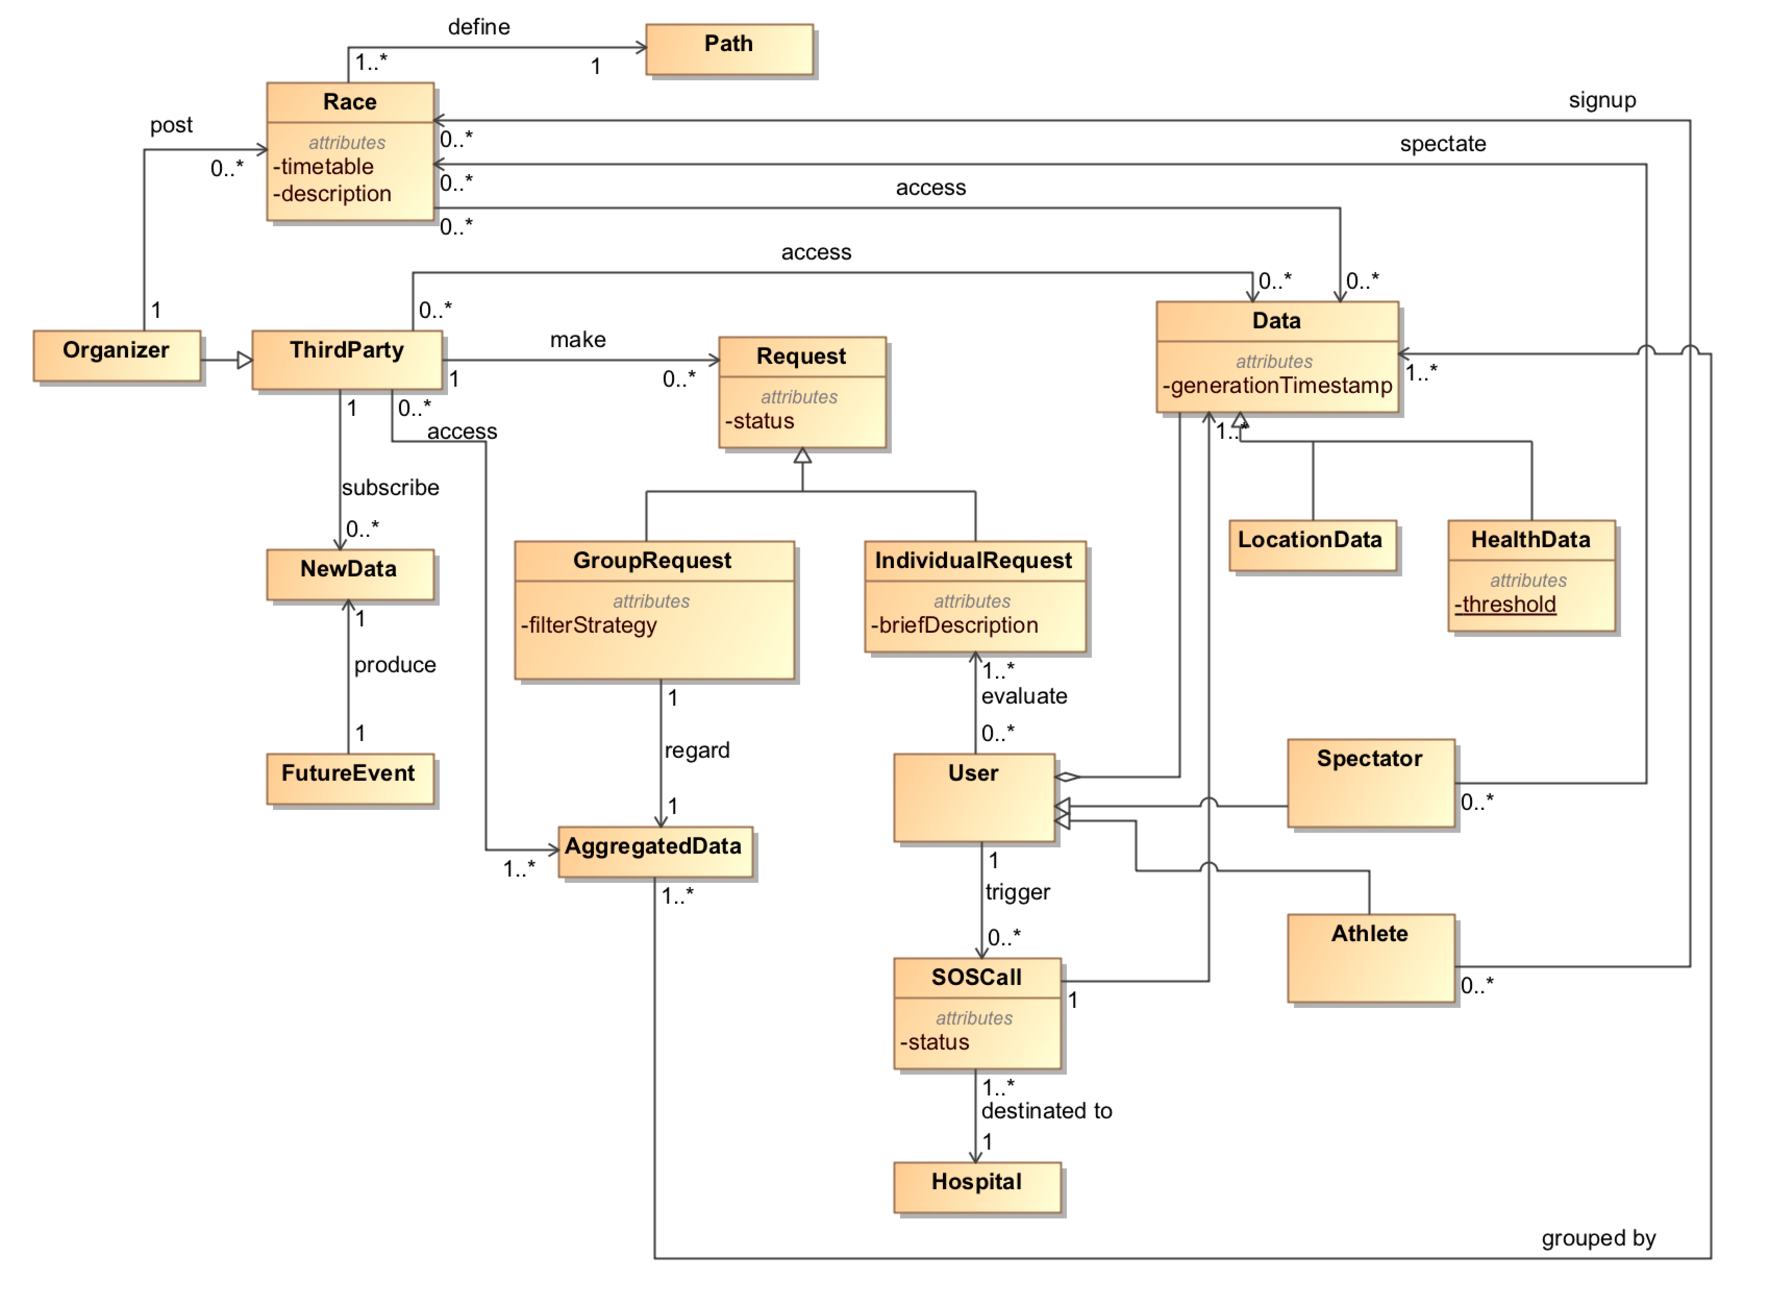
\includegraphics[width=\linewidth]{Images/classdiagram}
\caption{Class diagram of the environment}
\label{fig:classdiagram}
\end{figure}

This diagram specifies the interaction with the actors and the objects of the world. The core point of 
the environment is the data, but what should be analyzed are its entry and exit points (i.e. usage):

\begin{enumerate}
\item Request: an entry point essential to share the data;
\item SOSCall: a very important feature for unhealthy people;
\item Race: necessary for runners.
\end{enumerate}

\subsubsection{Request perspective}
Since people's data are very confidential information, a request has to be asked if someone desires it. 
Therefore, the design of how requests should work is essential. To give a better understanding of this, 
the following state diagram (Figure: \ref{fig:requestdiagram})  describes the possible states of a request:

\begin{figure}[H]
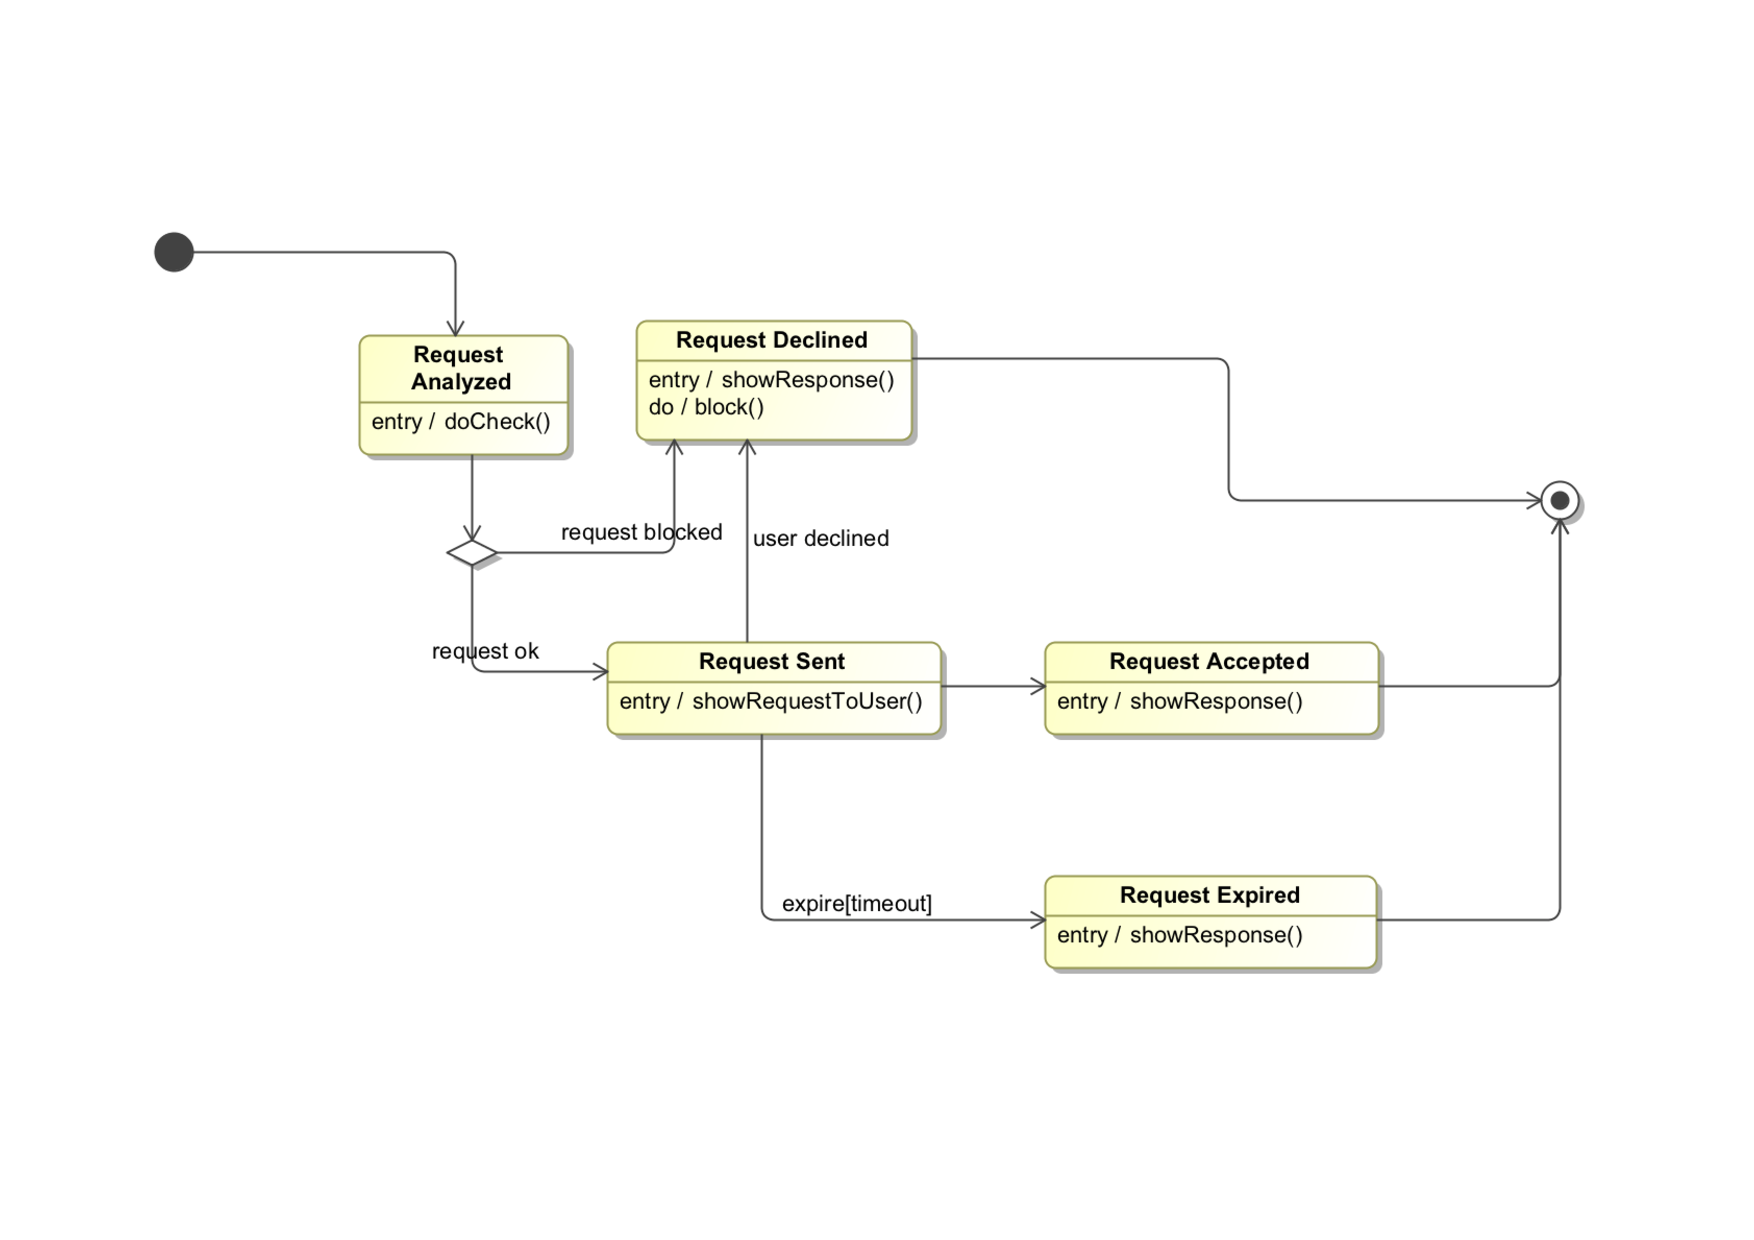
\includegraphics[width=0.8\linewidth]{Images/requestdiagram}
\caption{State diagram of a request}
\label{fig:requestdiagram}
\end{figure}

\subsubsection{SOSCall perspective}
For unhealthy people, a latency in a help call is a problem of life and death. Therefore, a better 
description of these calls is crucial. The following state diagram (Figure: \ref{fig:sosdiagram}) 
describes the possible states of a SOSCall:

\begin{figure}[H]
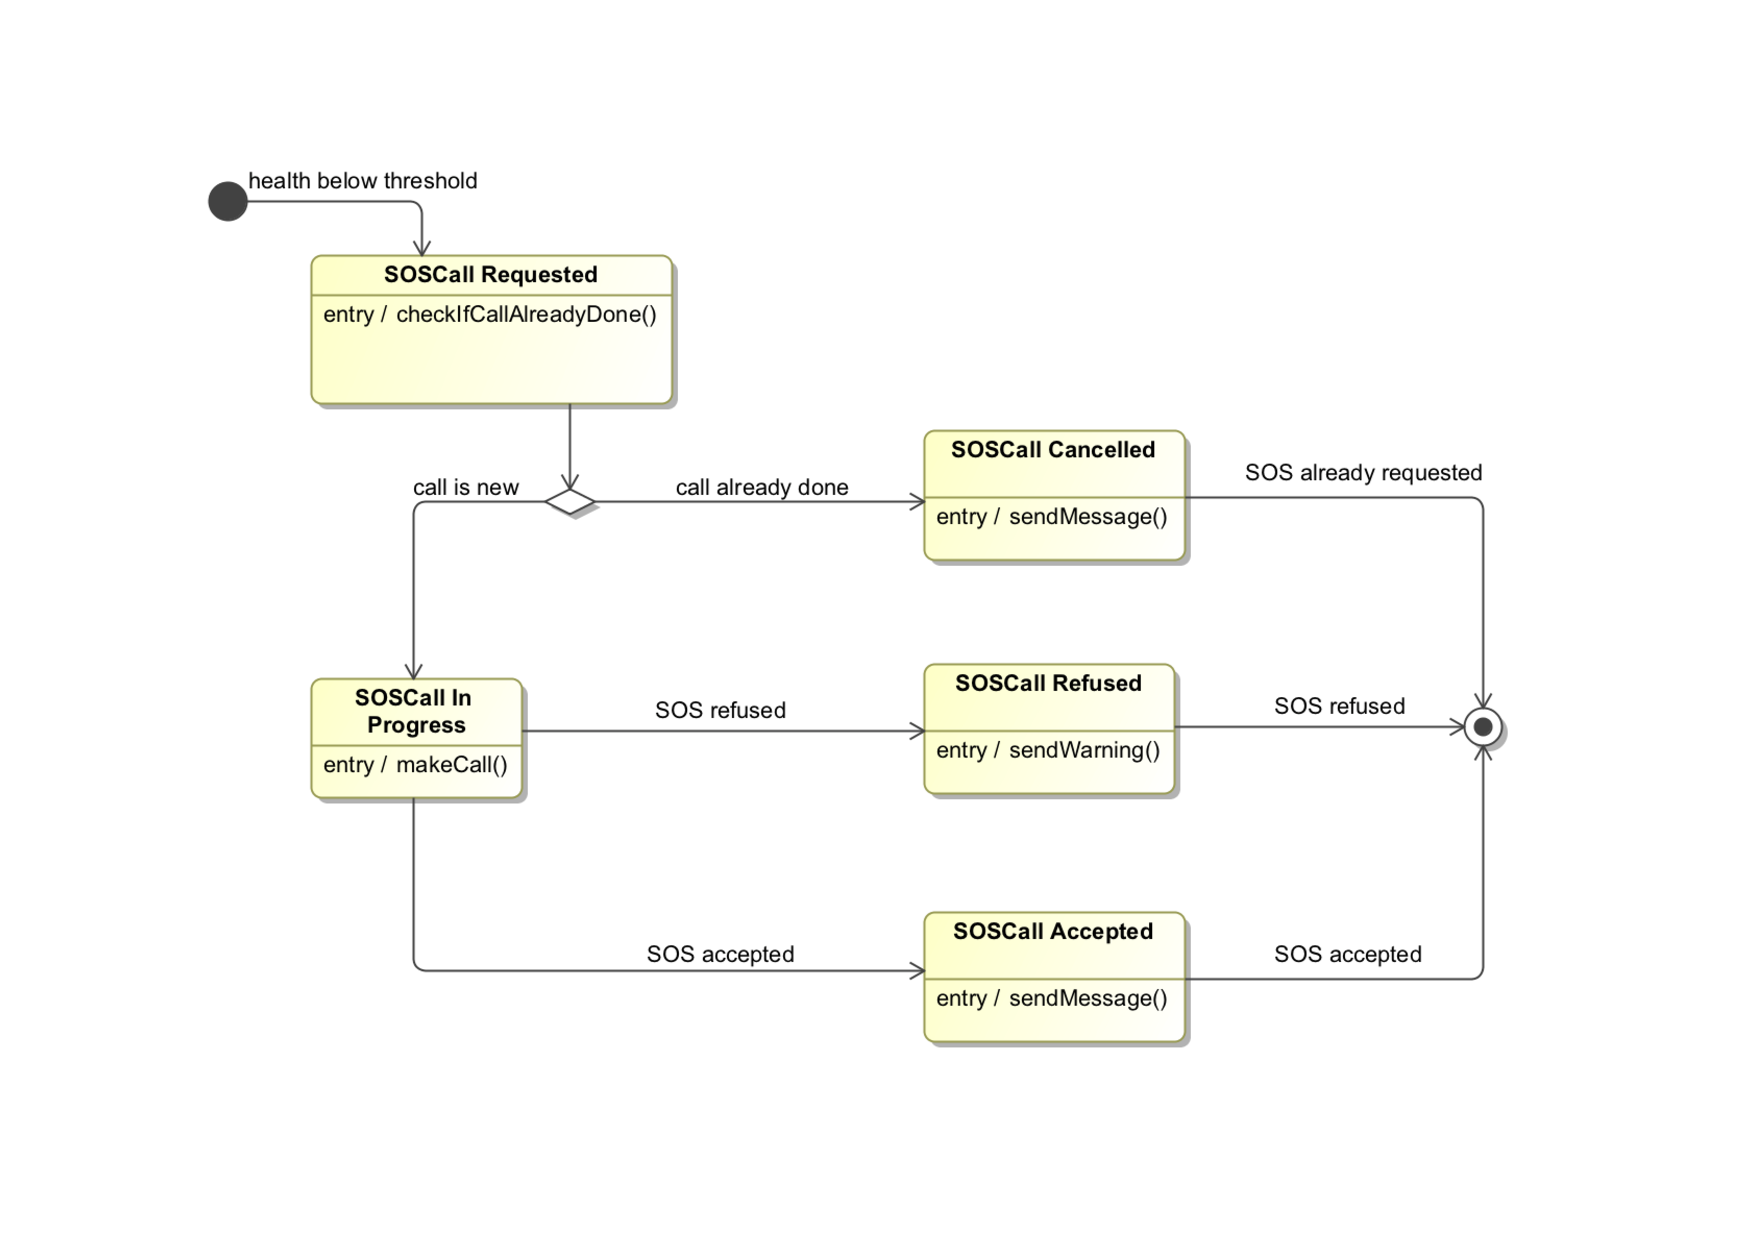
\includegraphics[width=0.8\linewidth]{Images/sosdiagram}
\caption{State diagram of a SOSCall}
\label{fig:sosdiagram}
\end{figure}

\subsubsection{Race perspective}
For someone, running is something that they cannot live without; since spectators can watch their 
position every time, it is important to describe better how a race works for better privatization of 
data. Thus, the following state diagram (Figure: \ref{fig:racediagram}) is shown: 

\begin{figure}[H]
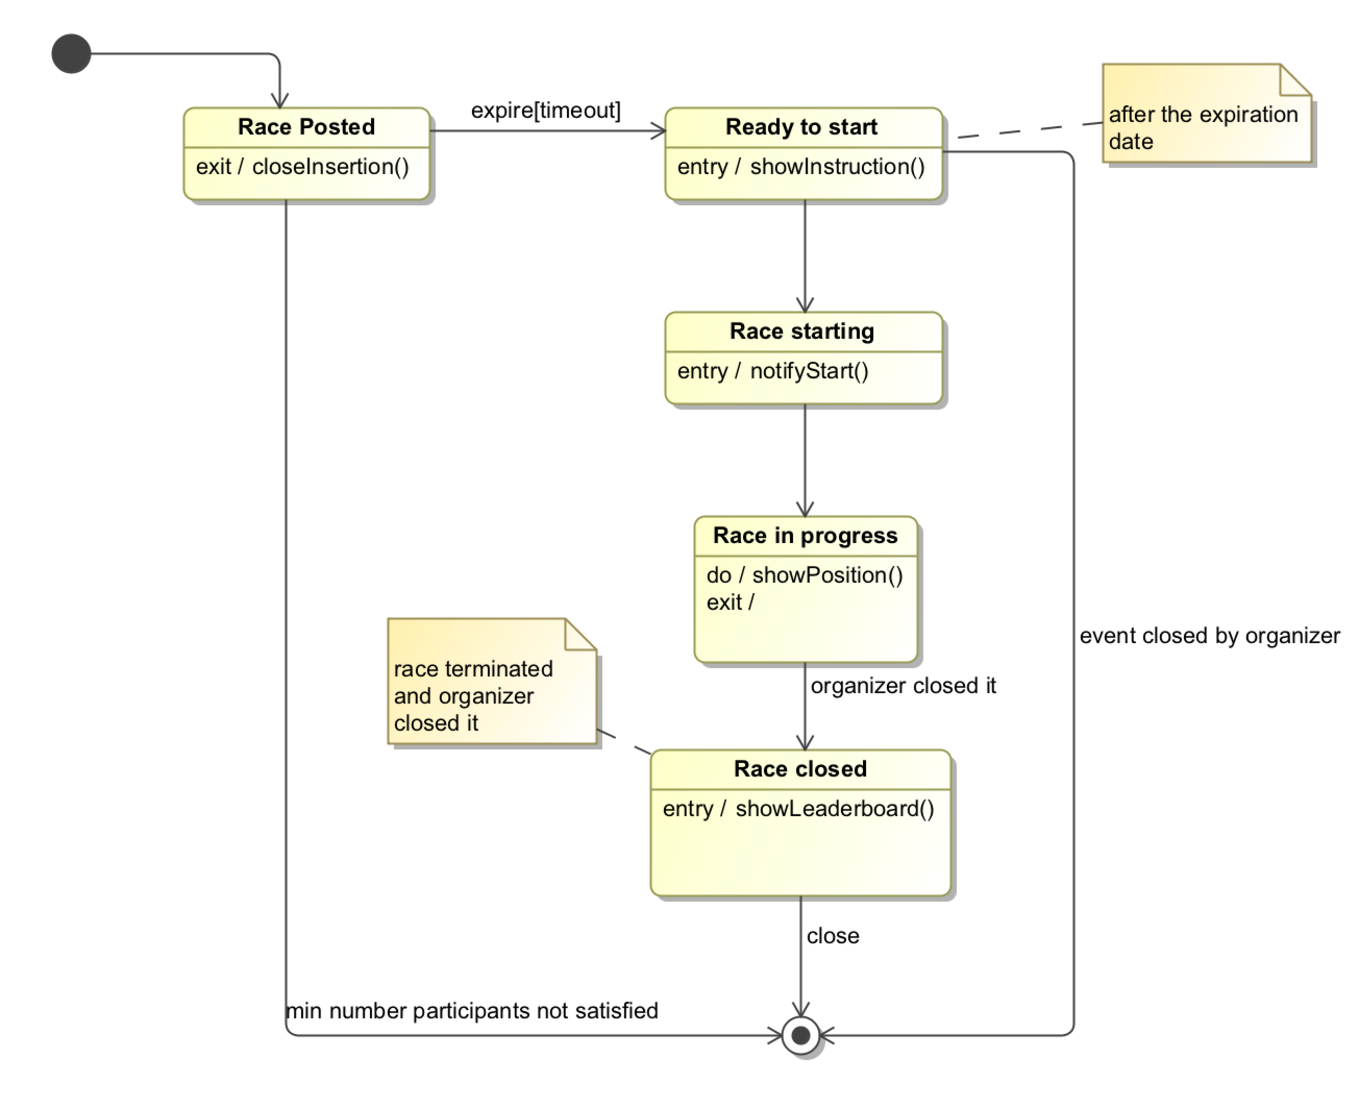
\includegraphics[width=0.8\linewidth]{Images/racediagram}
\caption{State diagram of a race}
\label{fig:racediagram}
\end{figure}
\subsection{Product functions}
\subsection{User characteristics}
\subsection{Assumptions, dependecies and constraints}

\subsubsection{Domain assumptions}
\begin{itemize}
\item[{[D1]}] User's smartphones are equipped with GPS sensor
\item[{[D2]}] Users own devices with sensors to acquire data information about health status
\item[{[D3]}] Health data collected by the devices are correct
\item[{[D4]}] There is at least an external service of trusted companies which provides the possibility to the user to view detailed maps
\item[{[D5]}] There is at least an external service of trusted companies which provides the possibility to make automated calls
\item[{[D6]}] There is at least an external service of trusted companies which provides the possibility to transfer data from devices containing sensors to acquire health data to smartphones
\item[{[D7]}] Everyone has a method to access for the first time to services offered by TrackMe
\item[{[D8]}] Hospitals always accepts new SOSCall regarding a person which has not yet received help.
\item[{[D9]}] If SOSCall are accepted, then an ambulance is sent to the location mentioned by the call
\item[{[D10]}] The service which shows the map of the world offers only paths that are feasible.
\item[{[D11]}] When a user's phone GPS is set on high precision, then it provides the right position with at most a radius error ranged from 0 to 10 meters
\item[{[D12]}] Athlete participating in a run are equipped with a device sharing GPS position set on high precision
\item[{[D13]}] After receiving help from an ambulance, a person can't be discharged before an hour
\item[{[D14]}] Every user enrolled in a run are able to participate in the run as athletes if all starting conditions are satisfied
\item[{[D15]}] All the organizers close a race that has not been canceled due to starting conditions
\end{itemize}


\newpage

\section{Specific Requirements}

\subsection{External interface requirements}
\subsubsection{User interfaces}
This section puts focus on the relation between the user and the mobile application. For better understanding the functionality of the application and the interaction with the user, beneath there are some mockups that represent a basic idea of what the mobile app will look like.

\begin{center}
\begin{minipage}[c]{.40\textwidth}
\centering
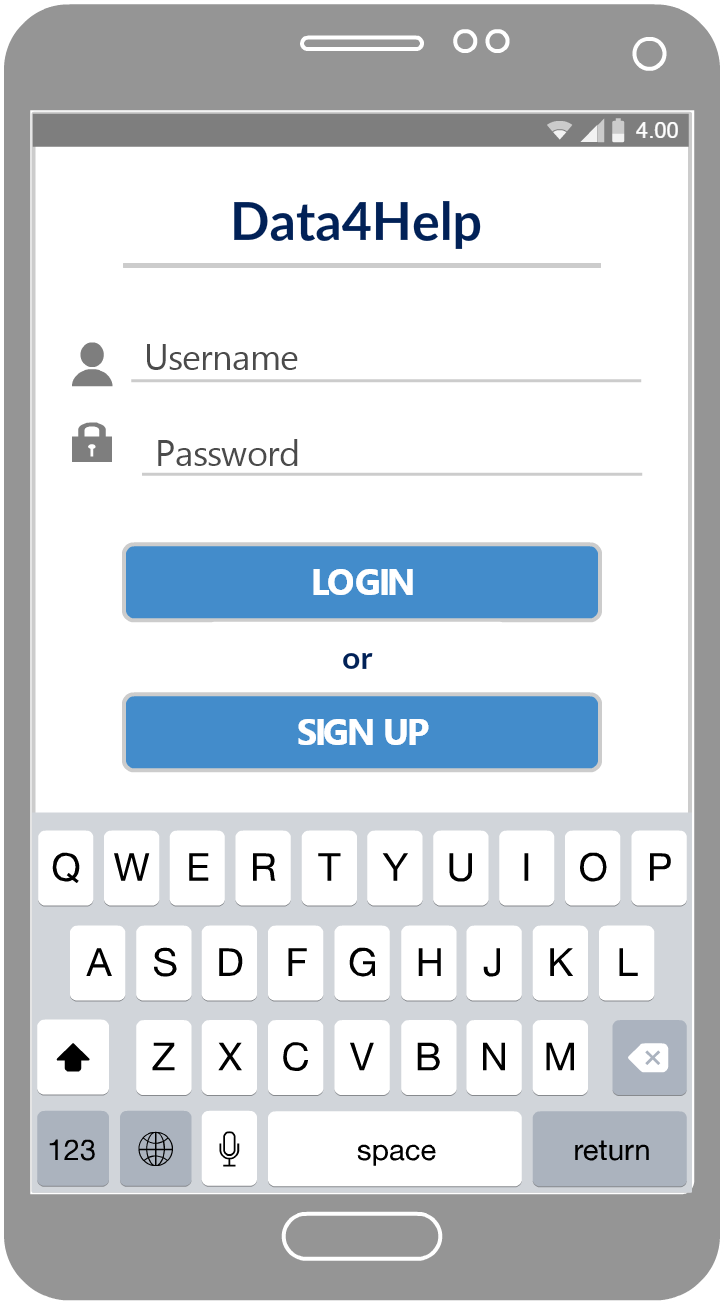
\includegraphics[width=1\textwidth]{Images/userInterface/Login}
\captionof{figure}{Mock up: Login.}
\end{minipage}%
\hspace{10mm}%
\begin{minipage}[c]{.40\textwidth}
\centering
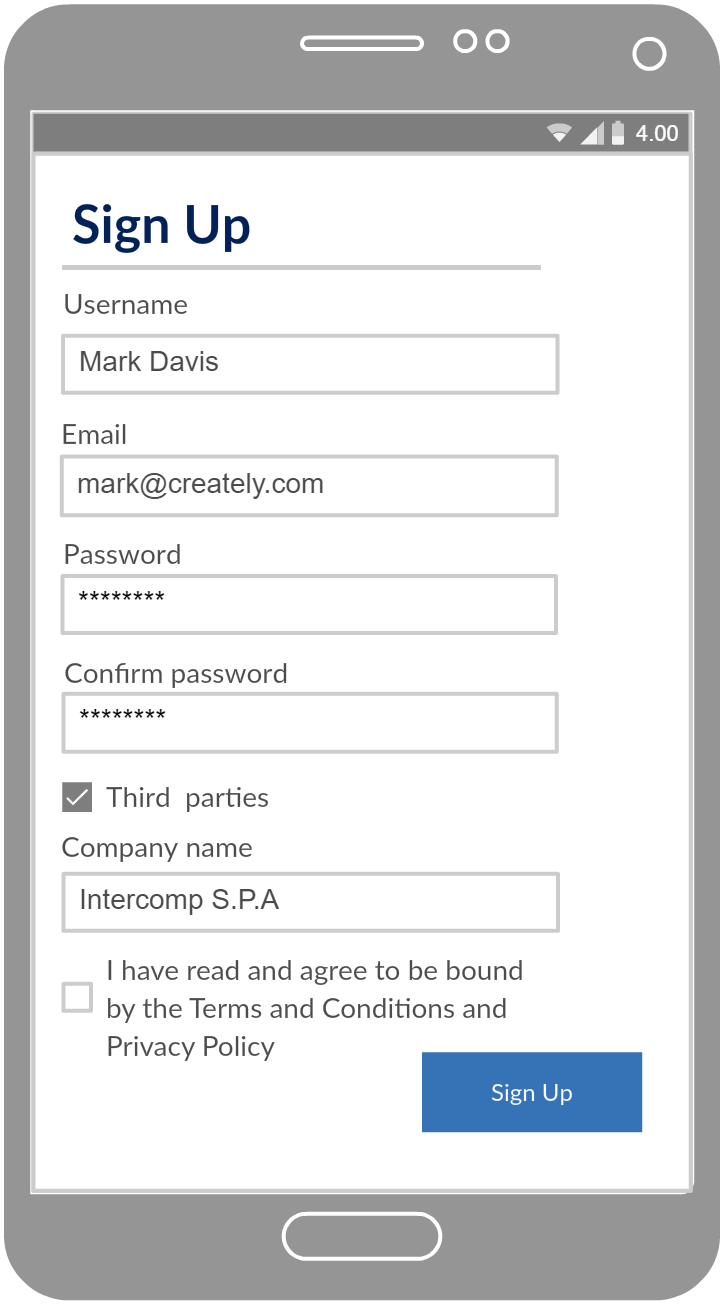
\includegraphics[width=1\textwidth]{Images/userInterface/SignUp}
\captionof{figure}{Mock up: Sign up.}
\end{minipage}
\end{center}
  
\begin{center}
\begin{minipage}[c]{.40\textwidth}
\centering
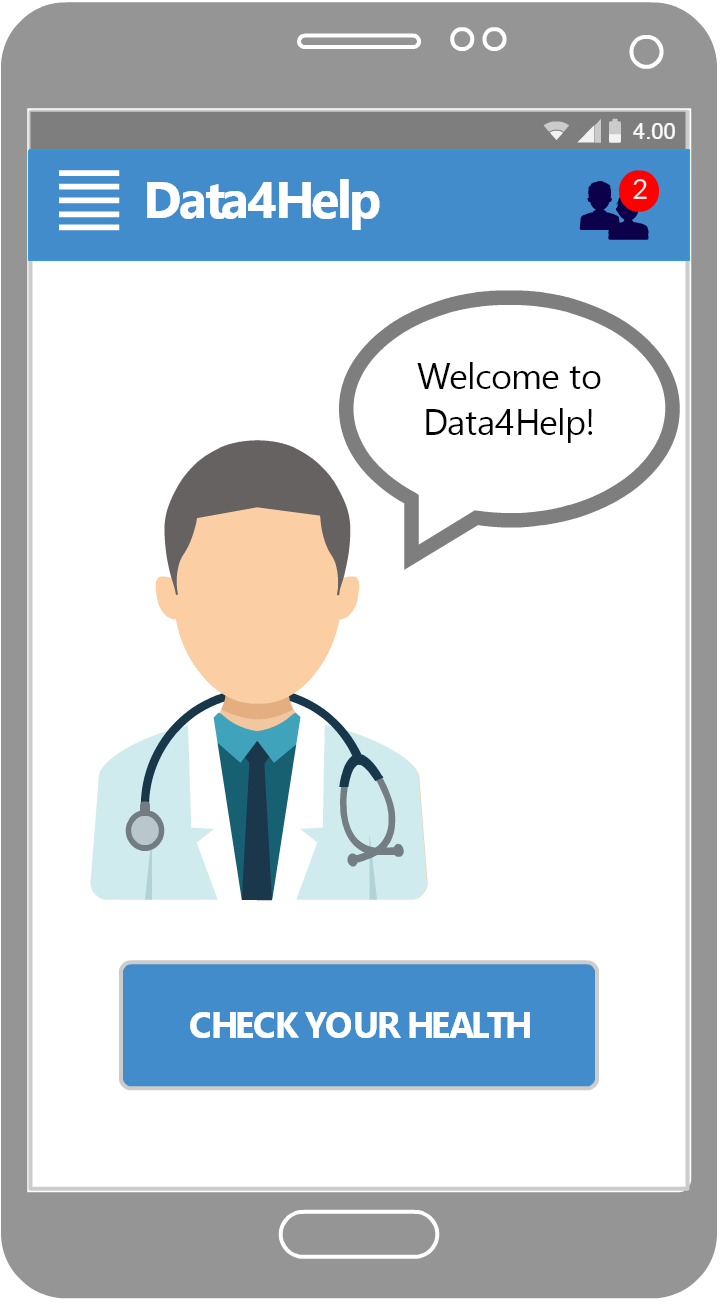
\includegraphics[width=1\textwidth]{Images/userInterface/Home}
\captionof{figure}{Mock up: Home.}
\end{minipage}%
\hspace{10mm}%
\begin{minipage}[c]{.40\textwidth}
\centering
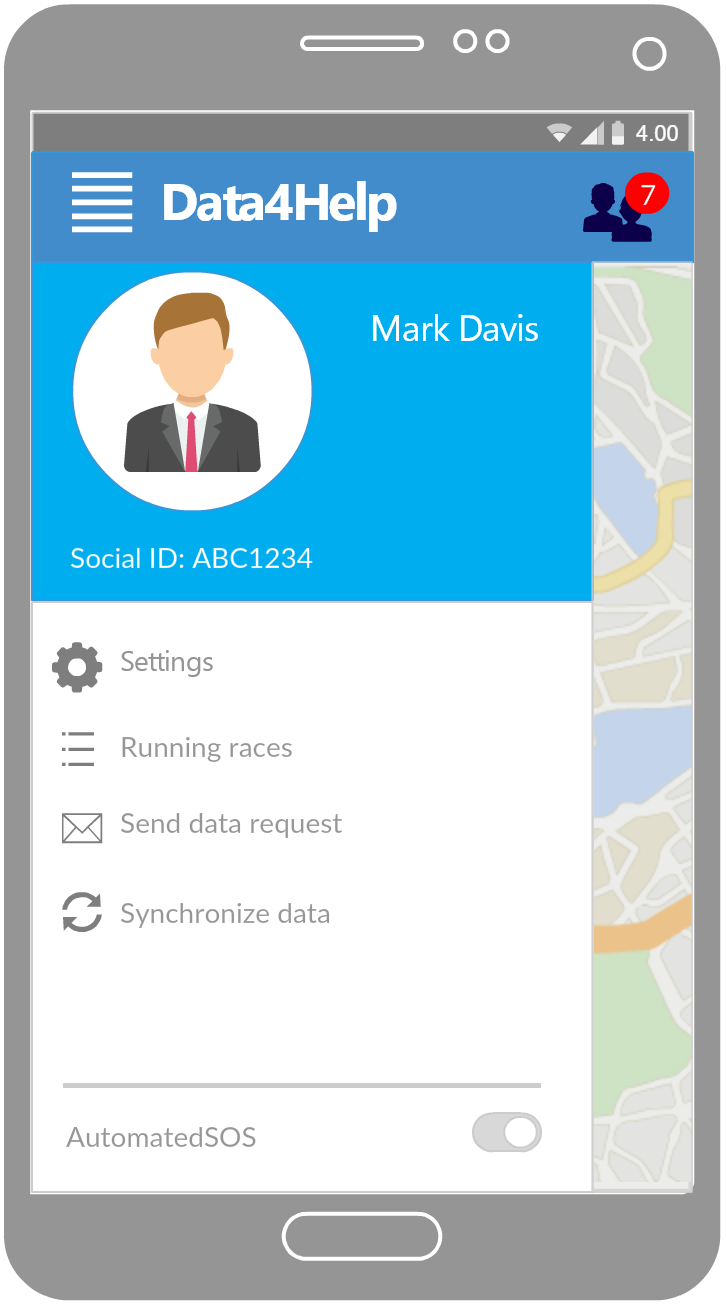
\includegraphics[width=1\textwidth]{Images/userInterface/MainMenu}
\captionof{figure}{Mock up: Main menu.}
\end{minipage}
\end{center}

\begin{center}
\begin{minipage}[c]{.40\textwidth}
\centering
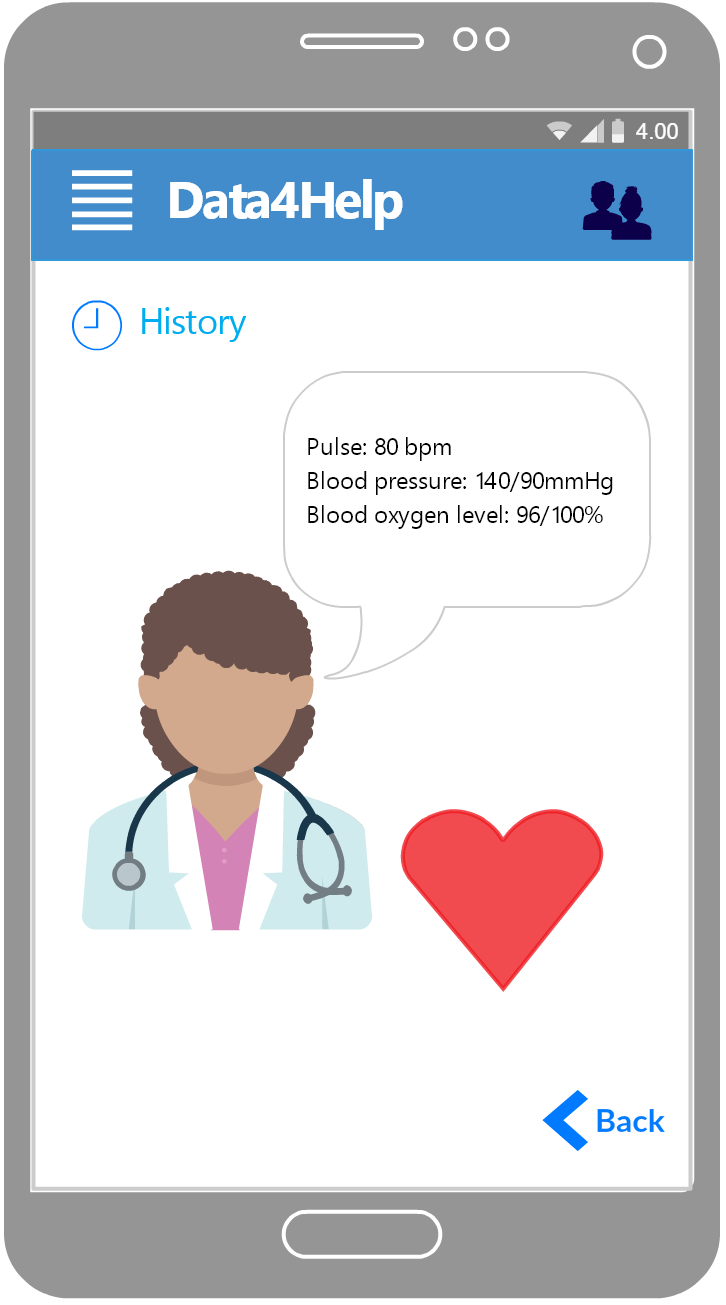
\includegraphics[width=1\textwidth]{Images/userInterface/HealthStatus}
\captionof{figure}{Mock up: Health status.}
\end{minipage}%
\hspace{10mm}%
\begin{minipage}[c]{.40\textwidth}
\centering
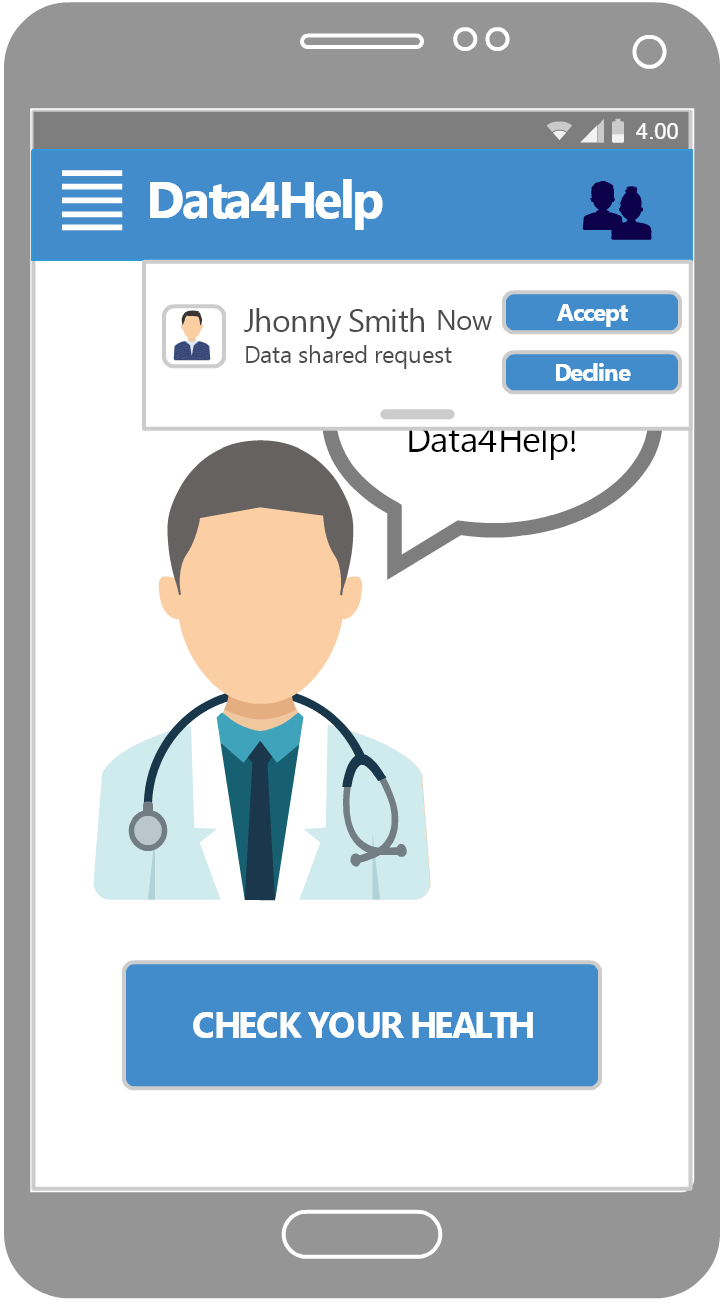
\includegraphics[width=1\textwidth]{Images/userInterface/ManageRequest}
\captionof{figure}{Mock up: Manage the request.}
\end{minipage}
\end{center}

\begin{center}
\begin{minipage}[c]{.40\textwidth}
\centering
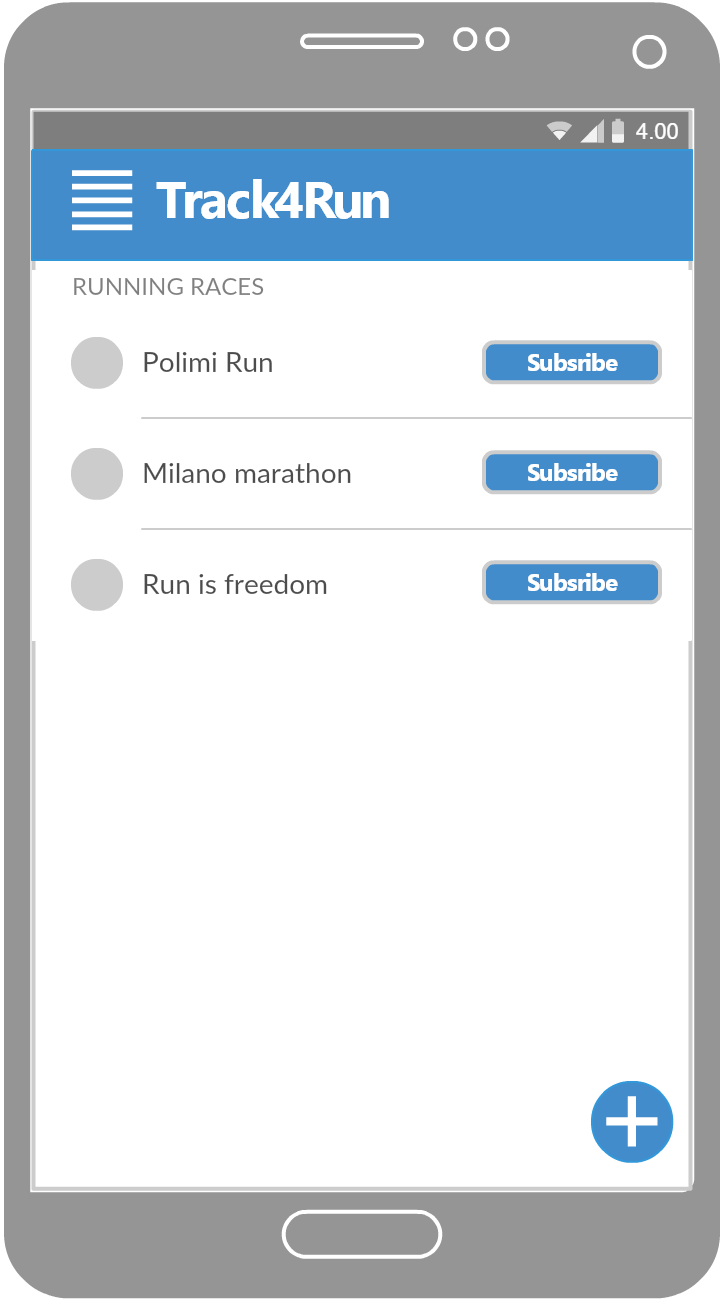
\includegraphics[width=1\textwidth]{Images/userInterface/RaceList}
\captionof{figure}{Mock up: List of available races.}
\end{minipage}%
\hspace{10mm}%
\begin{minipage}[c]{.40\textwidth}
\centering
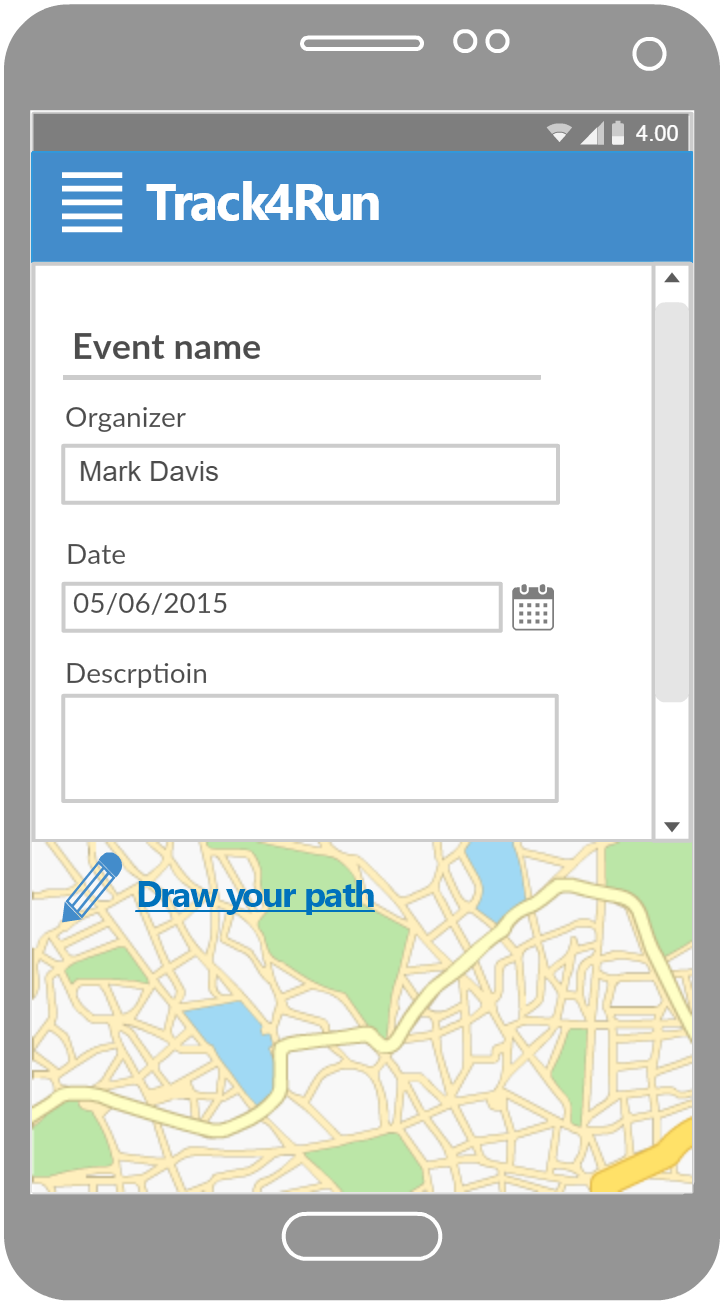
\includegraphics[width=1\textwidth]{Images/userInterface/AddEvent}
\captionof{figure}{Mock up: Add some events.}
\end{minipage}
\end{center}

\begin{center}
\begin{minipage}[c]{.40\textwidth}
\centering
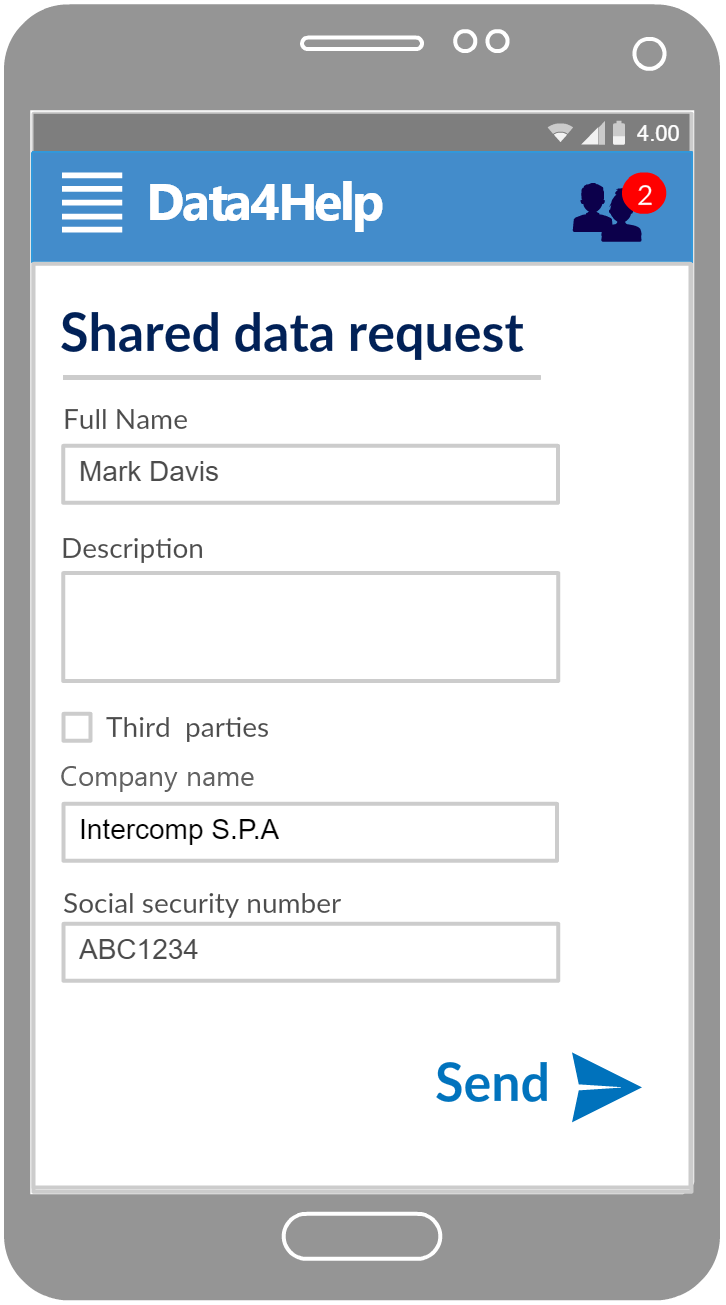
\includegraphics[width=1\textwidth]{Images/userInterface/SendRequest}
\captionof{figure}{Mock up: Shared data request form.}
\end{minipage}%
\hspace{10mm}%
\begin{minipage}[c]{.40\textwidth}
\centering
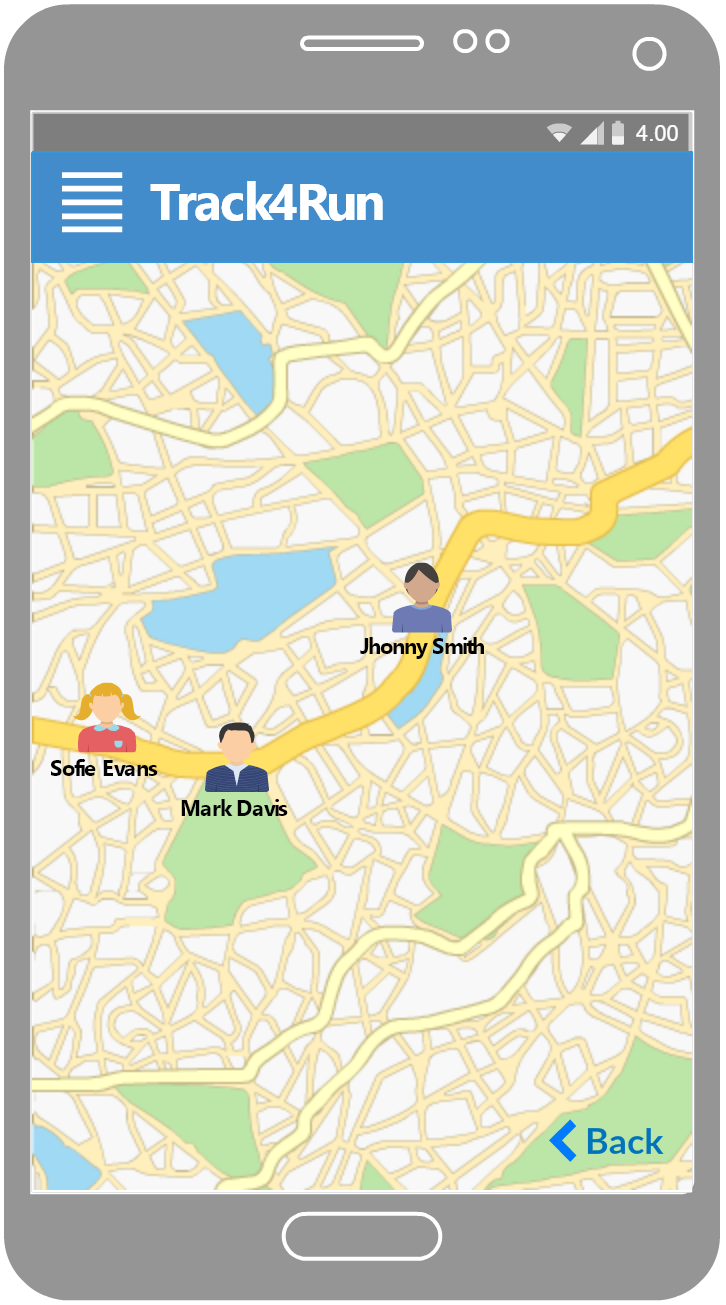
\includegraphics[width=1\textwidth]{Images/userInterface/Race}
\captionof{figure}{Mock up: Competition view.}
\end{minipage}
\end{center}
\subsubsection{Hardware interfaces}
To exploit the functionality of TrackMe services is mandatory to have two distinct hardware components:
\begin{enumerate}
\item First, it is necessary to own a smartphone which is used to interact with the mobile application;
\item Second, it is also essential to have a device provided with at least one NFC sensor: this has the ability to acquire heartbeat, blood pressure and blood oxygen saturation levels data.
\end{enumerate}
The latter, other than data acquisition, is also able to communicate with the smartphone in order to send the data acquired.\\
\begin{figure}[h!]
  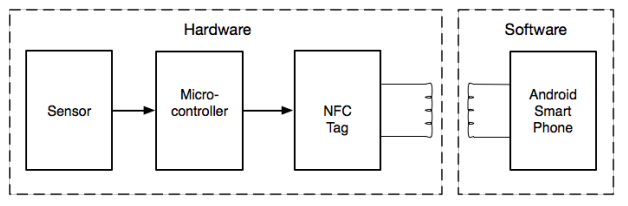
\includegraphics[width=\linewidth]{Images/hardware}
  \caption{The System Architecture.}
  \label{fig:The System Architecture}
\end{figure} 
The smartphone must also have a GPS system to provide the position, a monitor to allow, during the race, to see the athletes on the path, and finally the phone must be able to call the emergency room number.

\subsubsection{Software interfaces}
The application uses external services to reduce the product complexity:
\begin{enumerate}
\item Race map\\
The application requires a usage of map to define a path for the race and to see the position of the runner, during the competition. One options here is using Google Maps API which lets to customize maps with owner content and imagery for display on mobile devices. 
\item Call service\\
The smartphone's call service installed on the device is used by the application due to call the emergency number.
\item GPS Data service\\
The GPS Data as a Service API allows developers to store, handle, and manage GPS data in the system. It also analyzes GPS data in real time so that application can use it to provide the position during the call to the emergency room operator and during the running race. It can also provide reports on analyzed data. 
\item Automated call\\
Automated call service allows, to AutomatedSOS, to call the emergency number and to speak with the operator.
For instance, an option to recognize the answer provided by the emergency room operator could be the Google Cloud Speech API, that enables the AutomatedSOS feature to convert audio to text by applying neural network models in an easy to use API. 
\item Text-to-speech\\
The Text-to-Speech API is ideal for any application that plays audio of human speech to users. It allows the application to convert arbitrary strings, words, and sentences into the sound of a person speaking the same things. For example, in this case the API is used to read a formatted text message during the call to the emergency number. The message provides all the information that usually are required by the health staff. One possible API for this interface can be Google Text-to-speech.
\end{enumerate}
\subsubsection{Communication interfaces} 
The project needs several communication interfaces:
\begin{enumerate}
\item A communication interface to read/write data from the NFC tag. Fortunately, this already exists and it is called NFC protocol.
\item A communication interface to send and receive data over the network, in order to interact with the TrackMe system. One possible solution is to use the protocol HTTPS, that guarantees data security during upload and download operations. 
\item A communication interface to perform calls. 
\item A communication interface that exploit the GPS technology
\end{enumerate} 

\subsection{Scenarios}

\subsubsection{Scenario 1}
The company Canpari, whose business regards the production of natural and herbal medicines, needs data on the health statuses, during the last year, of the inhabitants of Milan. This will allow them to evaluate the project of opening their first shop in the city. \\
Therefore, with their Data4Help account, the marketing office compiles and sends an aggregated request for accessing the needed information. 
Once that the demand is received, the system analyses it: since there are, of course, more then a thousand of user subscribed in Milan, the requests is approved and the access is granted to Canpari. 

\subsubsection{Scenario 2}
The company Tibaldi\&Zhou has set up a shocking outdoor art show that will take place in the following two months in Piazza Duomo.
Therefore, it is interested in having access to data regarding the health statuses of the user that visit this location when they are close to the exhibition.
This is necessary in order to monitor the public feedback, using the heart rate of possible spectators. \\
In order to accomplish this purpose, they subscribes, using Data4Help, to the mentioned above future data: when the two months will pass by, the system will evaluate the anonymisation constraint. Since there will have been, of course, at least 1000 user that pass from Piazza Duomo, the access will be provided to the company. 

\subsubsection{Scenario 3}
Jacob is preparing for a marathon and, while training, he always keeps with him his device with the application installed. 
Unfortunately, yesterday he had an hearth attack while running, but his device was able to detect the health parameters below the threshold and have suddenly called the nearest hospital. \\
Once the call had been picked up, the device has communicated autonomously to the emergency room operator the observed health status and the location of the user, in order to request for an ambulance. 
Since, the operator understood the dangerous situation, he has accepted the demand and sent an ambulance to the location.

\subsubsection{Scenario 4}
The Company Like wants to organize a public run in Milan and it assigns this task to Mattia, who is the chief of the public relations office. \\
Therefore, Mattia opens the TrackMe's application and fill the form for submitting a new run event. 
More specifically, he defines the name of the run, its path, the date and the time in which the run will start, and a closure date for the subscriptions. 
Furthermore, he also specifies 10 as the minimum number of people that needs to be present.

\subsubsection{Scenario 5}
TangTang and his 9 nine friends are amateur runners that want to join a run in order to get some fun. 
Therefore, they decide to enroll, before the expiration date, in a run, whose minimum number of athletes is 10, organized by Abibas on the 5th of November. \\
When the expiration date arrives, the system checks the constraints on the number of runners. 
Since this constraint is satisfied, they wait the day of the event: at this point they race and, at the end of the competition, TangTang is announced as the winner. 


\newpage

\section{Formal Analysis using Alloy}
In the alloy model, in order to be safer w.r.t. the requirements that have been stated in this document, critical aspects have been modeled. 
In particular, the following vital goals have been asserted:
\begin{enumerate}
\item[{[G14]}]  Allow a third party to access data specified in a request if the user accepts the request or if he accepted one or more requests from the same third party that provided access to the same data 
\item[{[G15]}] Allow a third party to access statistical and anonymized data if and only if the number of individual involved is greater than 1000. This is satisfied as soon as the request is approved  
\item[{[G3]}] Once the health parameters of a user have been observed below the threshold for the first time after one hour, an ambulance is sent to the user location
\end{enumerate}

Notes that for G15, the fact that the aggregated request is satisfied as soon as the it is approved, is not been proven: the part considered critical is the access to the demanded information. \\

\lstinputlisting[language=alloy]{Alloy/trackme.als}

\newpage

\section{Effort Spent}

\subsection{Riccardo Poiani}

\begin{table}[H]
\begin{tabularx}{\textwidth}{|l|X|c|}
\hline
\rowcolor[HTML]{C0C0C0} 
Date & Task & Hours\\ \hline
15/10 & Goal definitions & 2.5\\ \hline
17/10 & Document structure, goal definition, class diagram & 2.5\\ \hline
18/10 & state diagram, class diagram, purpose, hypothesis & 1.5\\ \hline
19/10 & Scope, purpose and state diagram & 2\\ \hline
22/10 & Product functions & 2\\ \hline
23/10 & Scenarios & 2\\ \hline
24/10 & Scenarios & 1\\ \hline
25/10 & Refactor all document (revising) & 1\\ \hline
26/10 & Refactor all document (revising) & 4\\ \hline
27/10 & Add design standards, performance, availability, reliability, security; Add use case diagram and sequence diagram & 5\\ \hline
27/10 & Alloy & 2\\ \hline
28/10 & Alloy; world and shared phenomena; use case; whole document revision; sequence diagram & 7.5  \\ \hline
29/10 & Alloy; sequence diagram; fix requirement& 3 \\ \hline
01/11 & Revise document & 4 \\ \hline 
\rowcolor[HTML]{C0C0C0} 
& Overall & 40 \\ \hline
\end{tabularx}
\end{table}

\subsection{Mattia Tibaldi}

\begin{table}[H]
\begin{tabularx}{\textwidth}{|l|X|c|}
\hline
\rowcolor[HTML]{C0C0C0} 
Date & Task & Hours\\ \hline
15/10 & Goal definitions & 1.5\\ \hline
17/10 & Introduction & 2\\ \hline
18/10 & Scope and purpose & 4\\ \hline
19/10 & State diagram & 1\\ \hline
22/10 & Hardware interfaces & 2\\ \hline 
23/10 & Software interfaces & 3.5\\ \hline
24/10 & User interfaces & 3\\ \hline
25/10 & User interfaces and communication interfaces & 4\\ \hline 
27/10 & Revise document and use case & 3.5\\ \hline
28/10 & Alloy & 4.5\\ \hline
29/10 & Alloy and refactor document & 4\\ \hline
01/11 & Revise document & 4 \\ \hline 
\rowcolor[HTML]{C0C0C0} 
& Overall & 36\\ \hline
\end{tabularx}
\end{table}

\subsection{Tang-Tang Zhou}

\begin{table}[H]
\begin{tabularx}{\textwidth}{|l|X|c|}
\hline
\rowcolor[HTML]{C0C0C0} 
Date & Task & Hours\\ \hline
15/10 & Goal definitions & 2.5\\ \hline
17/10 & Document structure, goal definition, class diagram & 2.5\\ \hline
18/10 & state diagram, class diagram, purpose, hypothesis & 1.5\\ \hline
20/10 & Product Perspective, race diagram, request diagram and Alloy & 4\\ \hline
21/10 & Alloy & 1.5 \\ \hline
22/10 & Fix goals, purpose and perspective & 2\\ \hline
23/10 & Domain asssumptions and requirements & 2\\ \hline
24/10 & Requirements, goals, assumptions & 2\\ \hline
25/10 & Refactor all document (revising) & 2\\ \hline
26/10 & Refactor all document (revising) & 3\\ \hline
27/10 & Fix requirements, add alloy, add use case and sequence diagram & 5\\ \hline
27/10 & Add mantainability, portability, definitions, structure and references & 2\\ \hline
28/10 & Revise document, fix diagrams, add sequence diagram to document, add effort spent & 5\\ \hline
29/10 & Fix diagrams, Add alloy worlds, fix requirements & 2 \\ \hline
31/10 & sequence diagram & 1 \\ \hline
01/11 & Revise document & 3 \\ \hline 
\rowcolor[HTML]{C0C0C0} 
& Overall & 41\\ \hline
\end{tabularx}
\end{table}

\newpage

\end{document}
